\section{Results}
\label{sec:results}

To test the effectiveness of our new error term for rule extraction,
we applied our approach to six 
datasets from the UCI Machine Learning Repository \cite{uci}. Our
datasets are all classifications problems, covering a wide-range of
use-cases. \textit{Iris} is a classic classification dataset which
contains iris flower types and four associated length
measurements of the petal and sepal of the flower.
Both \textit{Yeast} and \textit{Ecoli}
record the localization site of a protein and a number of
physical measurements. \textit{Ionosphere} contains radar data collected
from high-frequency antennas and whether or not the collected data
contains evidence of the ionosphere. \textit{Seeds} describes three
varieties of wheat and geometrical properties of their kernels.
Finally, \textit{Waveform} describes three different types of waves
using 40 noisy measurements, where noise is generated normally
(with a mean of 0 and variance of 1).
An overview of our datasets is given in \ref{tab:datasets}.

We ran each dataset using two different approaches. The first
used only standard mean-squared error $E_1$
\footnote{Note that we use $E_1$ to refer to $E_1+E_3$ for simplicity, as
$E_3$ is included for both approaches}. The second used both
$E_1$ and our node separation term $E_2$. For each run, we recorded
the accuracy on the validation data and the $E_2$ error.
We first test to see if including $E_2$ in our error causes either
a significant decrease in accuracy or a significant increase
in $E_2$ hidden node separation. We then use C5.0 rule extraction
to assess if including $E_2$ leads to fewer rules generated.

\begin{table}[]
  \centering
\begin{tabular}{@{}llll@{}}
\toprule
Dataset             & Attributes & Classes & Samples \\ \midrule
\textit{Iris}       & 4          & 3       & 150     \\
\textit{Ecoli}      & 7          & 8       & 336     \\
\textit{Ionosphere} & 34         & 2       & 351     \\
\textit{Seeds}      & 7          & 3       & 210     \\
\textit{Waveform}   & 21         & 3       & 5000    \\ 
\textit{Yeast}      & 8          & 10      & 1484    \\ \bottomrule
\end{tabular}
\caption{UCI Machine Learning Datasets}
\label{tab:datasets}
\end{table}

There were a number of important design decisions for our networks
which we describe briefly below:

\begin{enumerate}
\item
  We tested every dataset on three different networks, with one,
  two, and three hiden layers respectively. Each hidden layer had
  four nodes \footnote{We used four as this is what was used in \cite{thuan11}}.
\item
  All weights in the networks were initialized by sampling from the
  uniform distribution from $[-1,1]$. Error backpropagation used RPROP
  to update weights.
\item
  $\beta$ values are critical to network performance. Thus, we automated
  tests to find $\beta$ values for each dataset and network using the
  following algorithm
  \begin{enumerate}
  \item
    Start $\beta$ at some reasonable upper limit ($0.01$).
  \item
    Use $\beta$ value to train four new networks. Also train four
    networks using only standard $E_1$ error.
  \item
    Assess accuracy of networks on testing data. If average accuracy
    across the four networks is greater than $0.05$ off of the average
    accuracy of the $E_1$ nets, repeat the process with
    $\beta = \frac{\beta}{2}$. If not, return $\beta$.    
  \end{enumerate}
  $\alpha$ simply initialized to $1-\beta$ after this process.
\item
  We set the weight decay factor $\lambda$ to 0.00001 as used in \cite{thuan11}.
\item
  In practice, despite the weight decay factor, some weights become large which
  can cause hidden node activations to be very close to $1$ ($1$ with floating
  point cutoff) regardless of the input. These nodes do not help cluster inputs
  and add unnecessary complication to rule extraction. Thus, for any node which
  reports an activation of $1$ for all validation data is pruned from the
  network.
\item
  We implemented early stopping to make training quicker. We use a simple
  method which stops after $100$ epochs if a new best accuracy on the
  training data has not been achieved. In practice, we found $100$ epochs is
  a big enough window that it does not significantly degrade performance.
  We run for a maximum of $400$ epochs.
\item
  $20\%$ of the data is reserved for validation, while the other $80\%$ is
  used for training. The data is randomly partitioned for each dataset and
  each network, but is kept the same for comparison of just $E1$ and $E1$
  with $E2$ for the same network/dataset.
\item
  Each network encodes outputs using standard one-hot encoding, where the number
  of output nodes is the number of classes, and the predicted class is the
  output node with the maximum activation.
\item
  We ran each dataset on each network 21 times. We computed both the average
  average validation error as well as the average node separation
  $-E_2/N^2$.
\end{enumerate}

It is important to note that some of the design decisions we
made do not directly correspond to the decisions made in the paper
that inspired this work~\cite{thuan11}. Because of this, it does not
make sense to directly compare our numerical results with theirs.
Thus we included single hidden layer
configurations in our experiment to create a control case that would
form the baseline for comparisons. 

We have recorded the average validation error and average node separation
for each dataset over the 21 runs in Table~\ref{tab:e1_e2_avgs}.
The large left column of results
gives the average validation error for both of the different errors
$E_1$ only and $E_1$ and $E_2$, and for $1$, $2$, and $3$ hidden layers.
The large right column of results
gives the average hidden node separation ($-E_2/N^{2}$)
for both of the different errors
$E_1$ only and $E_1$ and $E_2$, and for $1$, $2$, and $3$ hidden layers.
For each of the averages in the table, we compared performance with only the
$E_1$ error term and the $E_1$ and $E_2$ error term by performing a t-test
for statistically significant difference. We bolded each value in the table
that was determined significantly ($p < 0.05$) better.
In every case, including the $E_2$ error term
significantly increased the hidden node separation.
In twelve of the cases, average validation accuracy is significantly
better with only $E_1$, but only by a relatively small margin of
6\%. It should be noted that while the average margin of difference is
small, some datasets experienced rather large drops in accuracy. For instance,
\textit{Yeast} dropped by over 13\% for the two deeper network configurations.
These results show that, in many cases, adding in the $E_2$ error can
significantly increase hidden node separation while maintaining comparable
accuracy to networks with only $E_1$  error, but this is not always the
case as in \textit{Yeast} as $E_2$ separation can come at the cost of
accuracy.

We next discuss the results of the Rule Extraction experiments,
where we test how inclusion of the $E_2$ term affects the number
and accuracy of rules generated.
The results are
captured in Table~\ref{tab:re_results}, where the large second and
third columns
give the number of rule intervals and rule accuracy for each error term and
each network configuration of $1$, $2$, and $3$ hidden layers.
Once we trained networks for each dataset with
one, two, and three hidden layers, we ran 21 trials on each performing
rule extraction, reporting the mean of these runs. We report the
number of rule intervals generated instead of the number of network
rules because C5.0 tends to reports at maximum one rule for each output
class, where the condition of each rule is a disjunction of some number
of different intervals over the inputs.

For most cases, the number of rule intervals decrease when we add
the $E_2$ error term. Additionally, the rule accuracy across all
datasets and configurations stayed around the same, or actually
increased, when $E_2$ was included. To discover if these results were statistically
significant, we ran paired t-tests on the change in rule intervals
generated and as well as the change in rule accuracy. The standard
confidence level is 0.05, however the Bonferroni correction dictates
that when performing N tests \cite{shaffer1995multiple}, the confidence level should change according
to:
\begin{equation}
  \alpha = \frac{\alpha}{N}
\end{equation}
We run tests for all five datasets with three configurations for both
rule intervals and rule accuracy, bringing N to 30. Therefore,
significance for us is defined as $p < 0.05 / 30 =
0.00167$. \ref{tab:pval_results} shows the p values calculated for each
test, with the statistically significant ones bolded. 

%On average, adding in the $E_2$ error term resulted in a
%\todo{compute average difference in percentage of rules between $E_1$
%and $E_2 once we know which are stat sig}
%percentage difference in rules generated.
There are five dataset configurations that decrease the number of
intervals statistically significantly with the addition of $E_2$, Ecoli with one
hidden layer, Waveform with two and three hidden layers, and Yeast
with two and three hidden layers. In
Figures~\ref{fig:waveform_3d_1}, \ref{fig:waveform_3d_2}, \ref{fig:waveform_3d_3} we
can see why we had this success in the \textit{Waveform} hidden activations
for the 3 layer network comparing just $E_1$ and $E_1$ with $E_2$.
For each hidden node, adding in $E_2$ successfully forces the activations
apart, making hyper-planes more successful in partioning classes. 

It is notable that
the Seeds dataset with two hidden layers and both the
Seeds and Yeast datasets with only one
hidden layer do not. This is interesting as both of these datasets
experienced significantly greater $E_2$ separation for all network
configurations as noted in Table~\ref{tab:e1_e2_avgs}. In order
to better understand these outliers, we visualize the hidden node
behaviour for a one-layer network of \textit{Seeds}
in Figures~\ref{fig:seeds_3d_1},\ref{fig:seeds_3d_2},\ref{fig:seeds_3d_3}.
As we can see, for each of the three runs adding $E_2$ did not help push apart
activations, but actually managed to make it harder to draw hyper-planes
to separate the classes.

\begin{figure*}
\minipage{0.32\textwidth}
  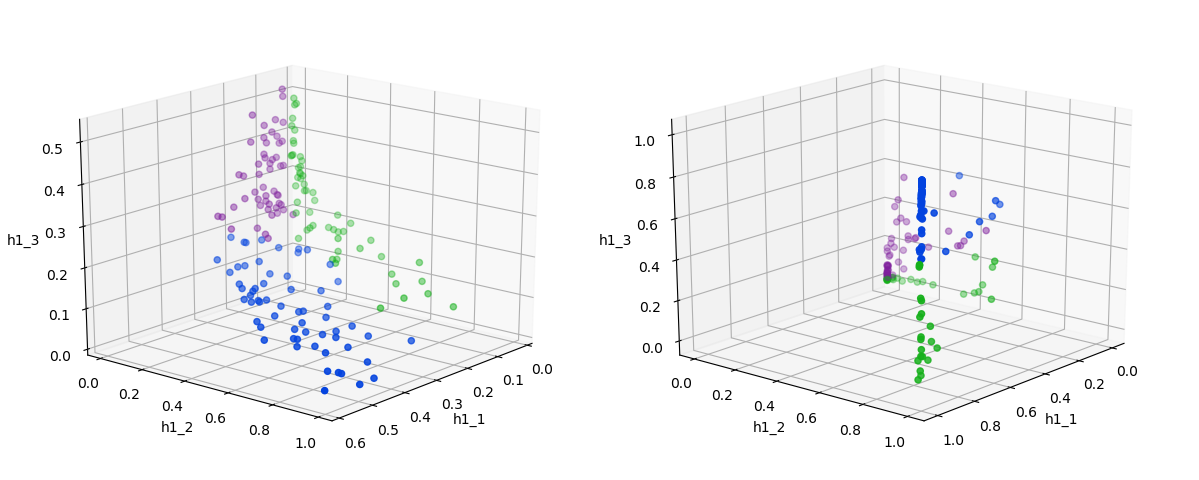
\includegraphics[width=\columnwidth]{4_h1_Seed_11_train_3d.png}
  \caption{\textit{Seeds} run 1 $E_1$ (left) vs. $E_2$ (right) hidden node activations}
    \label{fig:seeds_3d_1}
    \endminipage\hfill
\minipage{0.32\textwidth}
  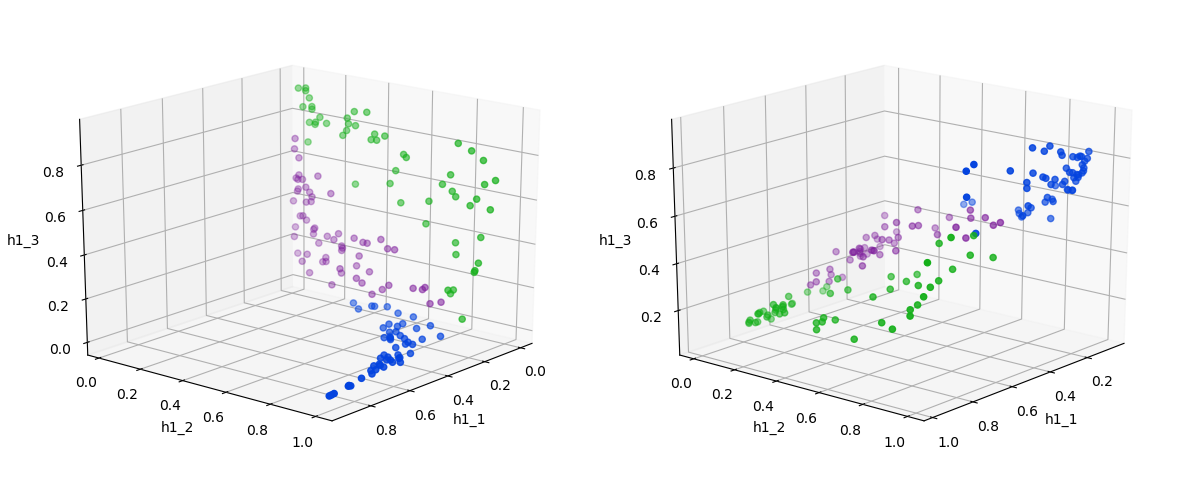
\includegraphics[width=\columnwidth]{4_h1_Seed_18_train_3d.png}
  \caption{\textit{Seeds} run 1 $E_1$ (left) vs. $E_2$ (right) hidden node activations}
    \label{fig:seeds_3d_2}
\endminipage\hfill
\minipage{0.32\textwidth}
  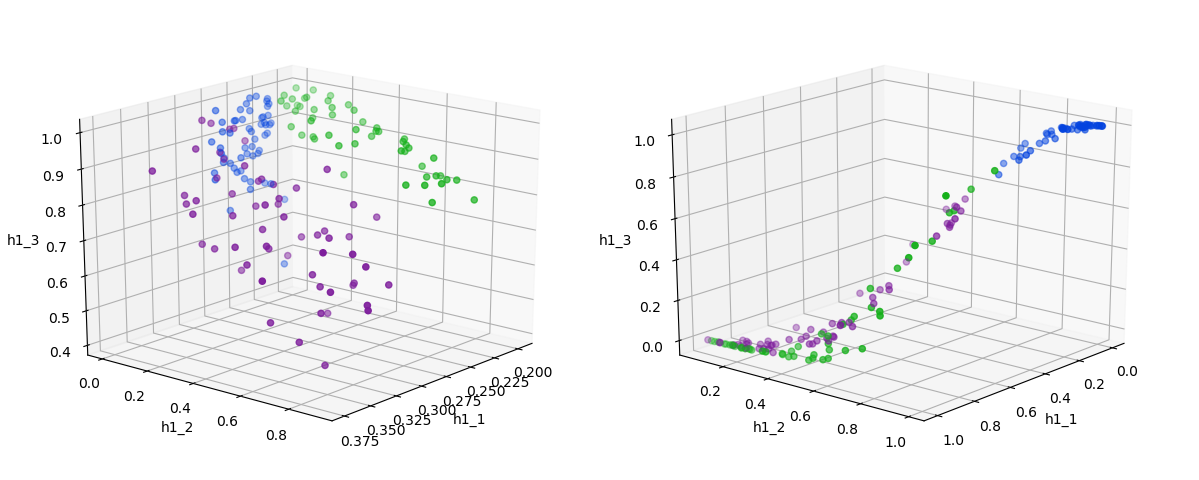
\includegraphics[width=\columnwidth]{4_h1_Seed_3_train_3d.png}
  \caption{\textit{Seeds} run 1 $E_1$ (left) vs. $E_2$ (right) hidden node activations}
    \label{fig:seeds_3d_3}
\endminipage
\end{figure*}

\begin{figure*} 
\minipage{0.32\textwidth}
  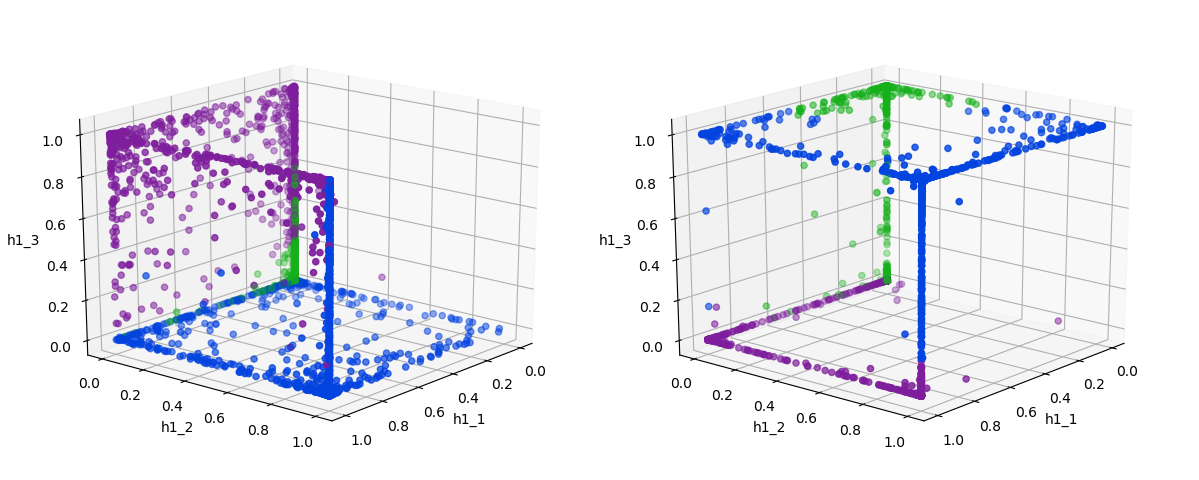
\includegraphics[width=\columnwidth]{4_4_4_h1_Seed_10_train_3d.png}
  \caption{\textit{Waveform} $E_1$ (left) vs. $E_2$ (right) hidden layer 1 activations}
  \label{fig:waveform_3d_1}    
    \endminipage\hfill
\minipage{0.32\textwidth}
  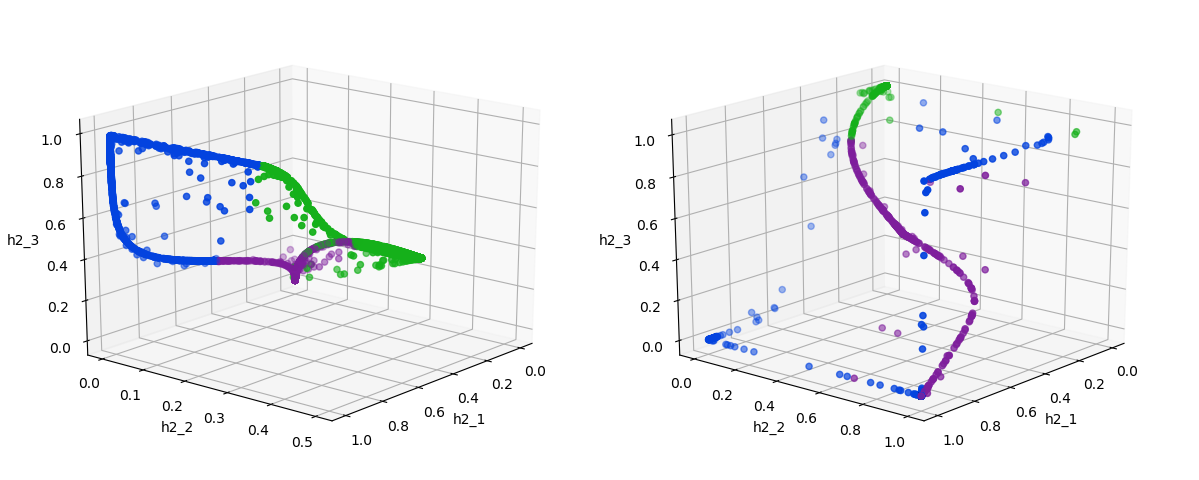
\includegraphics[width=\columnwidth]{4_4_4_h2_Seed_10_train_3d.png}
  \caption{\textit{Waveform} $E_1$ (left) vs. $E_2$ (right) hidden layer 2 activations}
  \label{fig:waveform_3d_2}    
\endminipage\hfill
\minipage{0.32\textwidth}
  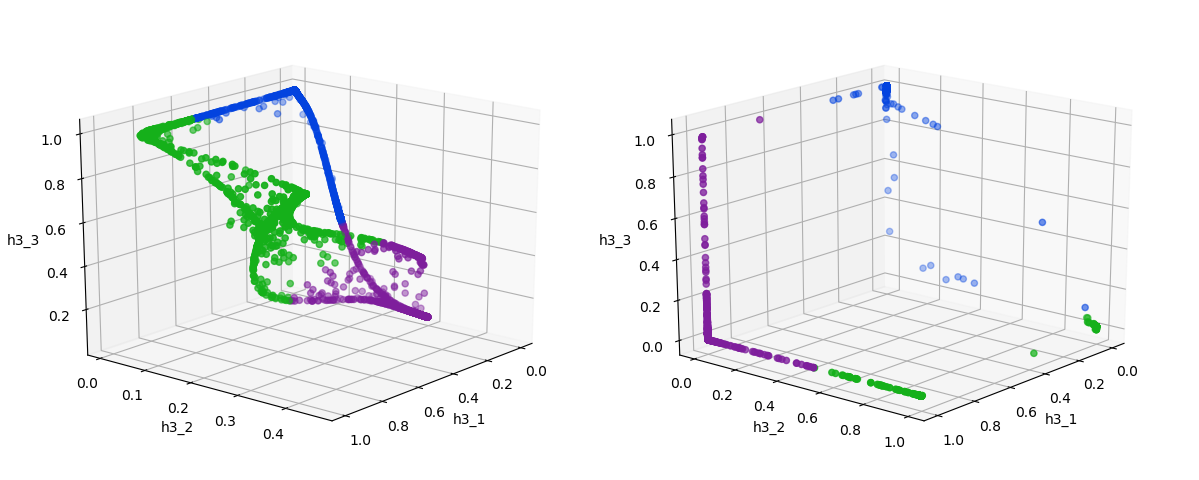
\includegraphics[width=\columnwidth]{4_4_4_h3_Seed_10_train_3d.png}
  \caption{\textit{Waveform} $E_1$ (left) vs. $E_2$ (right) hidden layer 3 activations}
  \label{fig:waveform_3d_3}  
\endminipage
\end{figure*}

Our generated rules are only an approximation of network behaviour,
thus it is important that we assess the accuracy of the generated rules.
If fewer rules were generated but those pruned rules
lost important context then the rules would actually be worse, not better.
For every single dataset and configuration, RE achieved
statistically similar ($p > 0.00167$) or statistically better ($p < 0.00167$)
rule accuracy with the $E_2$ term. This is most
notable in the Yeast datasets with two and three hidden layers, whose rule
accuracy increased by 25\% and 26\% respectively. This is especially interesting
as Yeast is one of the most difficult datasets to classify, with 10 output
classes that are not well separated. 

\begin{table*}[t!]
  \centering
  \small
  \begin{tabular}{|l|r|r|r|r|r|r|r|r|r|r|r|r|}
    \hline
    Dataset & 
    \multicolumn{6}{c|}{Avg Val Acc} & 
    \multicolumn{6}{c|}{$-2E_2/N^2$} \\
    \cline{2-13}
    & \multicolumn{3}{c|}{$E_1$ only} &
    \multicolumn{3}{c|}{$E_1$ and $E_2$} &
    \multicolumn{3}{c|}{$E_1$ only} &
    \multicolumn{3}{c|}{$E_1$ and $E_2$} \\
    \cline{2-13}
    & 1 & 2 & 3 & 1 & 2 & 3 & 1 & 2 & 3 & 1 & 2 & 3 \\
    \hline
    \textit{Iris} & \textbf{0.98} & \textbf{0.98} & 0.98 & 0.90 & 0.89 & 0.96 & 0.03 &0.08 & 0.10 & \textbf{0.07} & \textbf{0.10} & \textbf{0.13} \\
    \textit{Ecoli} & \textbf{0.85} & \textbf{0.83} & 0.79 & 0.73 & 0.78 & 0.79 & 0.01 & 0.05 & 0.07 & \textbf{0.05} & \textbf{0.09} & \textbf{0.10} \\
    \textit{Ionosphere} & \textbf{0.94} & \textbf{0.96} & 0.94 & 0.90 & 0.91 & 0.92 & 0.04 & 0.07 & 0.11 & \textbf{0.06} & \textbf{0.11} & \textbf{0.16} \\
    \textit{Seeds} & 0.88 & \textbf{0.89} & 0.86 & 0.85 & 0.85 & 0.84 & 0.01 & 0.03 & 0.06 & \textbf{0.04} & \textbf{0.06} & \textbf{0.09} \\
    \textit{Waveform} & \textbf{0.85} & \textbf{0.85} & \textbf{0.85} & 0.80 & 0.84 & 0.82 & 0.06 & 0.11 & 0.14 & \textbf{0.08} & \textbf{0.14} & \textbf{0.21} \\
    \textit{Yeast} & 0.57 & \textbf{0.57} & \textbf{0.55} & 0.57 & 0.44 & 0.43 & 0.02 & 0.03 & 0.05 & \textbf{0.04} & \textbf{0.10} & \textbf{0.17} \\
    \hline
  \end{tabular}
  \caption{Average Validation Accuracy and Hidden Layer Node Separation for Datasets}
  \label{tab:e1_e2_avgs}  
\end{table*}

\begin{table*}[t!]
  \centering
  %\small
  \begin{tabular}{|l|r|r|r|r|r|r|r|r|r|r|r|r|}
    \hline
    Dataset & 
    \multicolumn{6}{c|}{No. Rule Intervals} & 
    \multicolumn{6}{c|}{Rule Accuracy} \\
    \cline{2-13}
    & \multicolumn{3}{c|}{$E_1$ only} &
    \multicolumn{3}{c|}{$E_1$ and $E_2$} &
    \multicolumn{3}{c|}{$E_1$ only} &
    \multicolumn{3}{c|}{$E_1$ and $E_2$} \\
    \cline{2-13}
    \hline
    No. Hidden Layers & 1 & 2 & 3 & 1 & 2 & 3 & 1 & 2 & 3 & 1 & 2 & 3 \\
    \hline
    \textit{Iris} & 5.14 & 5.05 & 5.14 & 5.10 & 4.00 & 4.81 & 82.06\% &87.78\% & 92.38\% & 92.86\% & 90.10\% & 91.75\% \\
    \textit{Ecoli} & 109.00 & 106.67 & 94.05 &61.24 & 79.57 & 96.86 & 34.83\% & 53.94\% & 60.84\% & 59.84\% & 61.55\% & 58.28\% \\
    \textit{Ionosphere} & 39.55& 46.95& 45.55&30.86 & 37.86&
                                                             40.85&75.43\% & 84.79\%& 85.36\%&79.60\% & 87.82\%& 85.00\%\\
    \textit{Seeds} & 37.38 & 43.19 & 40.29 & 45.48 & 43.67 & 36.81 & 41.95\% & 55.67\% & 43.76\% & 42.18\% & 55.33\% & 46.26\% \\
    \textit{Waveform} & 1,748.35& 1,798.85 & 1,731.3 & 1,085.24 & 1,544.33 &
                                                                       1,341.05
                                  & 34.66\% & 50.18\%&49.19\% & 41.15\%&51.73\% & 56.14\%\\
    \textit{Yeast} &620.24 & 574.71& 553.05&704.43 & 353.81& 351.38&20.72\% & 41.32\%& 43.48\%&13.69\% &66.19\%&69.12\%\\
    \hline
  \end{tabular}
  \caption{Rule Extraction Results: Mean over 21 Runs}
  \label{tab:re_results}  
\end{table*}
%From Reggia: What were the findings?Visualizations for the results
\begin{table*}[t!]
  \centering
  %\small
  \begin{tabular}{|l|r|r|r|r|r|r|}
    \hline
    Dataset & 
    \multicolumn{3}{c|}{No. Rule Intervals} &
    \multicolumn{3}{c|}{Rule Accuracy} \\
    \cline{2-7}
    \hline
    No. Hidden Layers & 1 & 2 & 3 & 1 & 2 & 3 \\
    \hline
    \textit{Iris} & 0.9757 & 0.0733 & 0.5568 & 0.1997 & 0.5698 & 0.8836 \\
    \textit{Ecoli} & \textbf{8.465e-06} & 0.0134 & 0.7625 &\textbf{0.0009} & 0.0802 & 0.4761 \\
    \textit{Ionosphere} & 0.0140& 0.0210& 0.1414&0.0753 & 0.0291& 0.7931\\
    \textit{Seeds} & 0.0316 & 0.9319 & 0.6184 &0.9772 & 0.9481 & 0.6141 \\
    \textit{Waveform} & \textbf{1.91e-06}& 0.0118& \textbf{.0002} & 0.1087 & 0.4614 &0.0139\\
    \textit{Yeast} &0.0379 &\textbf{0.0002}&\textbf{0.0001}&0.0024 & \textbf{3.933e-06}& \textbf{1.292e-06}\\
    \hline
  \end{tabular}
  \caption{P-Values for t-Tests comparing E1 with E1 + E2}
  \label{tab:pval_results}  
\end{table*}
